\chapter{Encoding natural deduction}
\label{chap:ItL}

The sequent calculus encodings of chapters \ref{chap:sequentcalculus} and \ref{chap:sequentvariations} are each straightforward encodings of a logic, with a few directives to arrange the elements of the user interface. Natural deduction challenges us to allow forward reasoning steps. This chapter describes a first attempt: it can imitate only some kinds of forward step, and some features of the background tree are still traceable in the box display. The techniques described here are used in some later chapters, and in \chapref{I2L} a more polished attempt is described.

This encoding was used in a first-year course at QMW for several years, with increasing user satisfaction as the encoding more nearly approached the treatment used by the course lecturer. That lecturer chose the rules and, in particular, he chose to use a particular classical treatment of negation, not at all the one which I would have chosen myself, nor even the particular classical encoding which I would have preferred (see \chapref{I2L} for my own version).

The encoding is in \texttt{examples/ItL\_QMWpre2000}.

\begin{table}
\centering
\caption{Natural deduction rules in box form}
\label{tab:ItLboxrules}
\hstrut{5pt}\vstrut{5pt}\\
{\small
\begin{tabular}{|l|l|l|l|}
\hline
% ROW 1
$\begin{array}[b]{lll}
i: & A    &  \\
   & ...  &  \\
j: & A->B &  \\
   & ...  &  \\
k: & B    & \reason{$->-E\ i,j$}
\end{array}$
& 
$\begin{array}[b]{lll}
i: & A@B &  \\
   & ... &  \\
j: & A   & \reason{$@-E(L)\ i$}
\end{array}$
& 
$\begin{array}[b]{lll}
i: & A@B &  \\
   & ... &  \\
j: & B   & \reason{$@-E(R)\ i$}
\end{array}$
&
$\begin{array}[b]{lll}
i: & !!A &  \\
   & ... &  \\
j: & A   & \reason{$! -E\ i$}
\end{array}$
\\
\hline
\multicolumn{2}{|l|}{
$\begin{array}[b]{lll}
i: & A|B &  \\
   & ... &  \\
\begin{array}{@{}l}
j: \\
   \\
k:
\end{array}
		& 
		\begin{array}{|l|}
		\hline
		A \\
		... \\
		C \\
		\hline
		\end{array}
				& 
				\begin{array}{@{}l}
				\reason{assumption} \\
				\\
				\hstrut{5pt}
				\end{array}
\\
    & ... &  \\
\begin{array}{@{}l}
l: \\
   \\
m:
\end{array}
		& 
		\begin{array}{|l|}
		\hline
		B \\
		... \\
		C \\
		\hline
		\end{array}
				& 
				\begin{array}{@{}l}
				\reason{assumption} \\
				\\
				\hstrut{5pt}
				\end{array}
\\
   & ... &  \\
n: & C & \reason{$| -E\ i,j..k,l..m$}
\end{array}$}
&& \\
%ROW 3
\hline
\multicolumn{2}{|l|}{
$\begin{array}[b]{lll}
\begin{array}{@{}l}
\\
i: \\
\\
j: \\
\hstrut{5pt}
\end{array}
		& 
		\begin{array}{|l|}
		\hline
		... \\
		@*x.P(x) \\
		... \\
		P(c) \\
		... \\
		\hline
		\end{array}^{\;c}
				& 
				\begin{array}{@{}l}
				\\
				\hstrut{5pt} \\
				\\
				\reason{$@*-E\ i$} \\
				\hstrut{5pt}
				\end{array}
\end{array}$}
& 
\multicolumn{2}{|l|}{
$\begin{array}[b]{lll}
i: &|*x.P(x) &  \\
   & ... &  \\
\begin{array}{@{}l}
j: \\
\\
k:
\end{array}
		&
		\begin{array}{|l|}
		\hline
		P(c) \\
		... \\
		A \\
		\hline
		\end{array}^{\;c}
				& 
				\begin{array}{@{}l}
				\reason{assumption} \\
				\\
				\hstrut{5pt}
				\end{array}
\\
   & ... &  \\
l: & A & \reason{$|*-E\ i,j..k$}
\end{array}$}
\\
% ROW 4
\hline
\multicolumn{2}{|l|}{
$\begin{array}[b]{lll}
\begin{array}{@{}l}
i: \\
\\
j:
\end{array}
		& 
		\begin{array}{|l|}
		\hline
		A \\
		... \\
		B \\
		\hline
		\end{array}
				& 
				\begin{array}{@{}l}
				\reason{assumption} \\
				\\
				\hstrut{5pt}
				\end{array}
\\
   & ...  & \\
k: & A->B & \reason{$->-I\ i..j$} 
\end{array}$}
& 
\multicolumn{2}{|l|}{
$\begin{array}[b]{lll}
\begin{array}{@{}l}
i: \\
\\
j:
\end{array}
		& 
		\begin{array}{|l|}
		\hline
		A \\
		... \\
		B@!B \\
		\hline
		\end{array}
				& 
				\begin{array}{@{}l}
				\reason{assumption} \\
				\\
				\hstrut{5pt}
				\end{array}
\\
   & ... &  \\
k: & !A  & \reason{¬-I $i$..$j$}
\end{array}$}
\\
\hline
% ROW 5
$\begin{array}[b]{lll}
i: & A &  \\
& ... &  \\
j: & B &  \\
& ... &  \\
k: & A@B & \reason{$@-I\ i,j$}
\end{array}$
& 
$\begin{array}[b]{lll}
i: & A &  \\
& ... &  \\
j: & A|B & \reason{$| -I(L)\ i$}
\end{array}$
& 
$\begin{array}[b]{lll}
i: & B &  \\
& ... &  \\
j: & A|B & \reason{$| -I(R)\ i$}
\end{array}$
& \\
\hline
%ROW 6
\multicolumn{2}{|l|}{
$\begin{array}[b]{lll}
\begin{array}{@{}l}
\\
i:
\end{array}
		&
		\begin{array}{|l|}
		\hline
		... \\
		P(c) \\
		\hline
		\end{array}^{\;c}
				& 
\\
   & ...      &  \\
j: & @*x.P(x) & \reason{$@*-I\ i$} 
\end{array}$}
& 
\multicolumn{2}{|l|}{
$\begin{array}[b]{lll}
\begin{array}{@{}l}
\\
i: \\
\\
j: \\
\hstrut{5pt}
\end{array}
		& 
		\begin{array}{|l|}
		\hline
		... \\
		P(c) \\
		... \\
		|*x.P(x)) \\
		... \\
		\hline
		\end{array}^{\;c}
				& 
				\begin{array}{@{}l}
				\\
				\hstrut{5pt} \\
				\\
				\reason{$|*-I\ i$} \\
				\hstrut{5pt}
				\end{array}
\end{array}$}
\\
\hline
\end{tabular}
}
\end{table}

\newcommand{\vdotted}[1]{\begin{array}[b]{c}\vdots\\#1\end{array}}
\newcommand{\hvdotted}[2]{\begin{array}[b]{c}[#1]\\\vdots\\#2\end{array}}
\word{var,inscope}

\begin{table}
\centering
\caption{Natural deduction rules in tree form}
\label{tab:ItLtreerules}
\hstrut{5pt}\vstrut{5pt}\\
{\small
\begin{tabular}{|l|l|l|l|}
%ROW 0
\hline
\multicolumn{4}{|l|}{
$\infer[\reason{$hyp$}]
       {A}
       {}$}
\\
\hline
% ROW 1
$\infer[\reason{$->-E$}]
       {B}
       {\vdotted{A} \vdotted{A->B}}$
& 
$\infer[\reason{$@-E(L)$}]
       {A}
       {\vdotted{A@B}}$
& 
$\infer[\reason{$@-E(R)$}]
       {B}
       {\vdotted{A@B}}$
& 
$\infer[\reason{$\;!-E$}]
       {A}
       {\vdotted{!!A}}$
\\
\hline
\multicolumn{2}{|l|}{
$\infer[\reason{$| -E$}]
       {C}
       {\vdotted{A|B} & \hvdotted{A}{C} & \hvdotted{B}{C}}$}
&
\multicolumn{2}{|l|}{
$\infer[\reason{$@*-E$}]
       {P(c)}
       {\vdotted{@*x.P(x)} & c\;\<inscope>}$}
\\
\hline
% ROW 2
\multicolumn{4}{|l|}{
$\infer[\reason{(\textsc{fresh} $c$, $c$ \textsc{notin} $|*x.P(x)$) $|*-E$}]
       {A}
       {\vdotted{|*x.P(x)} & \hvdotted{\<var> c,P(c)}{A}}$}
\\
\hline
% ROW 3
$\infer[\reason{$->-I$}]
       {A->B}
       {\hvdotted{A}{B}}$
& 
$\infer[\reason{$@-I$}]
       {A@B}
       {\vdotted{A} & \vdotted{B}}$
& 
$\infer[\reason{$| -I(L)$}]
       {A|B}
       {\vdotted{A}}$
& 
$\infer[\reason{$| -I(R)$}]
       {A|B}
       {\vdotted{B}}$
\\
\hline 
% ROW 4
$\infer[\reason{$!-I$}]
       {!A}
       {\hvdotted{A}{B@!B}}$
&
$\infer[\reason{(\textsc{fresh} $c$) $@*-I$}]
       {@*x.P(x)}
       {\hvdotted{\<var> c}{P(c)}}$
& 
\multicolumn{2}{|l|}{
$\infer[\reason{$|*-I$}]
       {|*x.P(x)}
       {\vdotted{P(c)} & c\;\<inscope>}$}
\\
\hline
\end{tabular}}
\end{table}

\begin{table}
\centering
\caption{Natural deduction rules in sequent form}
\label{tab:ItLsequentrules}
\hstrut{5pt}\vstrut{5pt}\\
{\small
\begin{tabular}{|l|l|l|l|}
\hline
% ROW 0
\multicolumn{4}{|l|}{
$\infer[\reason{$hyp$}]
       {\Gamma,A |- A}
       {}$}
\\
\hline
% ROW 1
$\infer[\reason{$
\;->-E$}]
       {\Gamma  |- B}
       {\Gamma  |- A & \Gamma  |- A->B}$
& 
$\infer[\reason{$@-E(L)$}]
       {\Gamma  |- A}
       {\Gamma  |- A@B}$
& 
$\infer[\reason{$@-E(R)$}]
       {\Gamma  |- B}
       {\Gamma  |- A@B}$
& 
$\infer[\reason{$! -E$}]
       {\Gamma  |- A}
       {\Gamma  |- !!A}$
\\
\hline
% ROW 2
\multicolumn{2}{|l|}{
$\infer[\reason{$| -E$}]
       {\Gamma |- C}
       {\Gamma |- A|B & \Gamma,A |- C & \Gamma,B |- C}$}
& 
\multicolumn{2}{|l|}{
$\infer[\reason{$@* -E$}]
       {\Gamma  |- A(c) }
       {\Gamma  |- @*x.A(x)  & \Gamma |- c\;\<inscope>}$} 
\\ 
\hline
% ROW 3
\multicolumn{4}{|l|}{
$\infer[\reason{(\textsc{fresh} $c$, $c$ \textsc{notin} $|*x.A$) $|* -E$}]
       {\Gamma  |- B}
       {\Gamma  |-|*x.A(x)  & \Gamma ,\<var> c,A(c)  |- B}$
}
\\
\hline
% ROW 4
$\infer[\reason{$-> -I$}]
       {\Gamma  |- A->B}
       {\Gamma,A |- B}$
& 
$\infer[\reason{$@ -I$}]
       {\Gamma  |- A@B}
       {\Gamma  |- A & \Gamma  |- B}$
& 
$\infer[\reason{$| -I(L)$}]
       {\Gamma  |- A|B}
       {\Gamma  |- A}$
& 
$\infer[\reason{$| -I(R)$}]
       {\Gamma  |- A|B}
       {\Gamma  |- B}$
\\
\hline
% ROW 5 
$\infer[\reason{$\;!-I$}]
       {\Gamma  |- !A}
       {\Gamma,A |- B@!B}$
&
$\infer[\reason{(\textsc{fresh} $c$) ∀-I}]
       {\Gamma |- @*x.A(x) }
       {\Gamma,\<var> c |- A(c) }$
& 
$\infer[\reason{∃-I}]
       {\Gamma |-|*x.A(x) }
       {\Gamma  |- A(c)  & c\;\<inscope>}$
&\\
\hline
\end{tabular}}
\end{table}

\section{Inference rules}

The rules of natural deduction are not normally stated in terms of sequents. The rules were presented to me in box-and-line form as in \tabref{ItLboxrules} (there was also a reiteration rule, which I don't list).\footnote{If anybody knows how to make Latex lay out this table with adequate space before and after each row, and without picking some elements and jamming them up against the top of the box, please let me know.} The marginal $c$ in the ∃-E and ∀-I rules indicates a proviso that $c$ should not appear free outside the `scope box' which it labels; there's a corresponding condition on ∃-I and ∀-E that $c$ should be `well scoped' --- that is, lines $i$ to $j$ have to be inside a scope box for $c$.

These rules have well-known tree equivalents shown in \tabref{ItLtreerules}, where reiteration is replaced by a hypothesis rule, the provisos are made explicit and the ∃-I and ∀-E rules have an explicit side-condition. The provisos on ∃-E and ∀-I implement the provisos on the box rules reasonably accurately. They aren't quite the same, because there could be disjoint parts of the tree where the same name is used; in practice, because my encoding of these rules makes them introduce names new to the proof, the distinction is unnoticeable. To implement the condition on ∃-I and ∀-E I have used pseudo-predicates var and inscope; $c$ inscope is a side condition that var $c$ must occur in the hypotheses.

It's easy to recast these rules in sequent notation as in \tabref{ItLsequentrules}. Plainly it is a difficulty, in a backwards-reasoning tool, that these are all right-hand rules. Yet if we are to be satisfy to our client's requirements, these are the rules that we must encode. In order to understand how to do that, it is necessary to understand how they are intended to be used.

\section{Syntax (\texttt{ItL\_syntax.j})}

The description of the syntax differs only slightly from that used in the sequent calculus encodings of chapters \ref{chap:sequentcalculus} and \ref{chap:sequentvariations}. Quantification affects the \textit{smallest} following formula: that is, in this encoding $@*x.A->B$ should parse as $(@*x.A) ->B$.\footnote{Our customer also wanted no punctuation between bound variable and body: I've never found a way to make Jape's parser generator allow that.} The priority of quantification is therefore just less than that of negation.
\begin{quote}\tt\small
CLASS VARIABLE x y z c d \\
CLASS FORMULA A B C P Q R S \\
CLASS BAG FORMULA Γ \\

PREFIX  10      var \\
POSTFIX 10      inscope \\

INFIX       100R    → \\
INFIX       120L        ∨ \\
INFIX       140L        ∧ \\

LEFTFIX 180     ∀ . \\
LEFTFIX 180     ∃ . \\

PREFIX  200     ¬ \\
JUXTFIX 300 \\
SUBSTFIX    400  \\

BIND x SCOPE P IN ∀x . P \\
BIND x SCOPE P IN ∃x . P \\

SEQUENT IS BAG ⊢ FORMULA
\end{quote}

We set two variables (really they are parameters, because they can only be altered when the rule and theorem store is empty):
\begin{quote}\tt\small
INITIALISE autoAdditiveLeft true \\
INITIALISE interpretpredicatesbtrue
\end{quote}

The first of these allows us to define rules without mentioning a left context, automatically inserting a context variable \ensuremath{\Gamma} into every sequent in a rule definition (that is, allowing rule definition in the style of natural deduction and earlier versions of Jape). The second directs Jape to interpret every juxtaposition --- everything that looks like a predicate application --- as a predicate application, to translate where necessary into substitution notation and to include additional rule parameters and invisible provisos to support the translation.

\section{The rules in Japeish (\texttt{ItL\_rules.j})}

The introduction and elimination rules are exactly those of \tabref{ItLsequentrules}, all stated without repetition of the context Γ. \texttt{hyp} is \textsc{automatch}ed and an \textsc{identity} rule, just as in the sequent calculus.
\begin{quote}\tt\small
RULE "→-E"(A)      IS FROM A AND A→B INFER B \\
RULE "∧-E(L)"(B)   IS FROM A ∧ B INFER A \\
RULE "∧-E(R)"(A)   IS FROM A ∧ B INFER B \\
RULE "∨-E"(A,B)    IS FROM A ∨ B AND A ⊢ C AND B ⊢ C INFER C \\
RULE "¬-E"         IS FROM ¬¬A INFER A \\
RULE "∀-E"(c)      IS FROM ∀x. A(x) AND c inscope INFER A(c) \\
RULE "∃-E"(OBJECT c) WHERE FRESH c AND c NOTIN ∃x.A(x) \\
\tab IS FROM ∃x.A(x) AND var c, A(c) ⊢ C INFER C

RULE "→-I"         IS FROM A ⊢ B INFER A→B \\
RULE "∧-I"         IS FROM A AND B INFER A ∧ B \\
RULE "∨-I(L)"(B)   IS FROM A INFER A ∨ B \\
RULE "∨-I(R)"(A)   IS FROM B INFER A ∨ B \\
RULE "¬-I"(B)      IS FROM A ⊢ B ∧ ¬B INFER ¬A \\
RULE "∀-I"(OBJECT c) WHERE FRESH c \\
\tab IS FROM var c ⊢ A(c) INFER ∀x .A(x) \\
RULE "∃-I"(c)      IS FROM A(c) AND c inscope INFER ∃x.A(x) \\

RULE hyp(A) IS INFER A ⊢ A \\
AUTOMATCH hyp \\
STRUCTURERULE IDENTITY   hyp
\end{quote}

To imitate forward reasoning we need a \textsc{cut} rule; to use theorems easily we need a \textsc{weaken} rule.
\begin{quote}\tt\small
RULE cut(B) IS FROM B AND B ⊢ C INFER C \\
RULE thin(A) IS FROM C INFER A ⊢ C

STRUCTURERULE CUT        cut \\
STRUCTURERULE WEAKEN     thin
\end{quote}

To deal with variables we need a rule that picks up $\<var>$ declarations, and it's \textsc{automatch}ed too.
\begin{quote}\tt\small
RULE "inscope" IS INFER var x ⊢ x inscope \\
AUTOMATCH "inscope"
\end{quote}
(It is offensive to use the context in this way, as if $\<var> c$ was a logical assertion. Jape doesn't have structured contexts, more's the pity.)

\section{Variable settings (\texttt{ItL.jt})}

We don't want novices to apply a conjecture until it is proved, and we don't want the engine to use a resolution step unless a tactic commands it:
\begin{quote}\tt\small
INITIALISE applyconjectures false\\
INITIALISE tryresolution false
\end{quote}
The display style should be box-and-line, and we want to control the naming of assumptions: the outermost assumption should be ``premise'', plural ``premises'' (the \texttt{innerassumption} settings look like a hangover from an earlier version of Jape, as those are the defaults anyway):
\begin{quote}\tt\small
INITIALISE displaystyle box

INITIALISE outerassumptionword premise\\
INITIALISE outerassumptionplural premises\\
INITIALISE innerassumptionword assumption\\
INITIALISE innerassumptionplural assumptions
\end{quote}

\begin{figure} 
\centering 
\subfigure[problem statement]{\centering
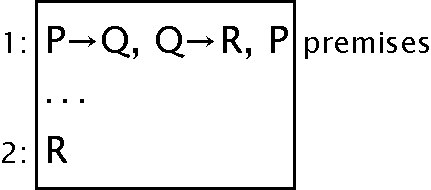
\includegraphics[scale=0.5]{pics/forwardstepA} \label{fig:forwardstepA}} 
\quad
\subfigure[hypothesis selected]{\centering
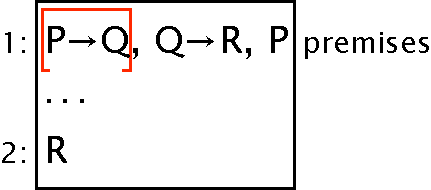
\includegraphics[scale=0.5]{pics/forwardstepB} \label{fig:forwardstepB}} 
\quad
\subfigure[after →-E]{\centering
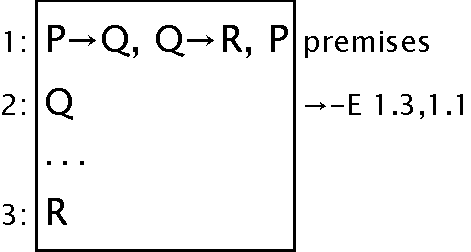
\includegraphics[scale=0.5]{pics/forwardstepC} \label{fig:forwardstepC}} 
\quad
\subfigure[second hypothesis selection]{\centering
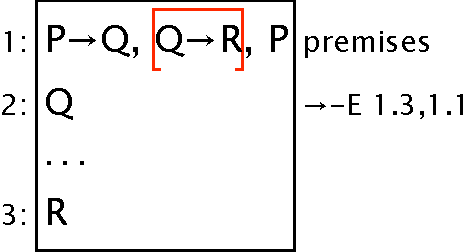
\includegraphics[scale=0.5]{pics/forwardstepD} \label{fig:forwardstepD}} 
\quad
\subfigure[second →-E completes proof]{\centering
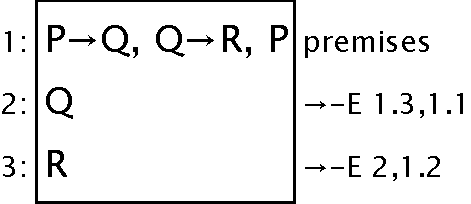
\includegraphics[scale=0.5]{pics/forwardstepE} \label{fig:forwardstepE}} 
\caption{A proof using forward steps}
\label{fig:forwardstep}
\end{figure}

\begin{figure} 
\centering 
\subfigure[after →-E]{\centering
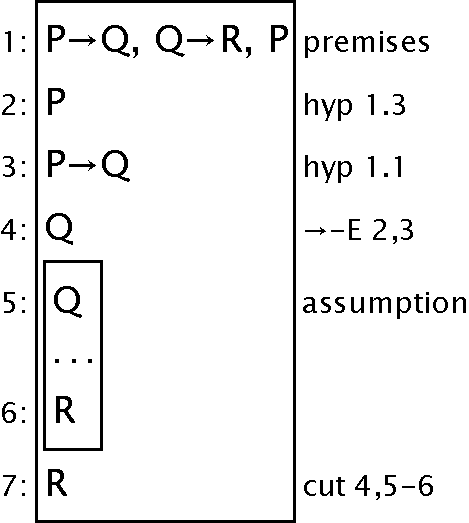
\includegraphics[scale=0.5]{pics/forwardstepwithcutC} \label{fig:forwardstepwithcutC}} 
\quad
\subfigure[tree after →-E]{\centering
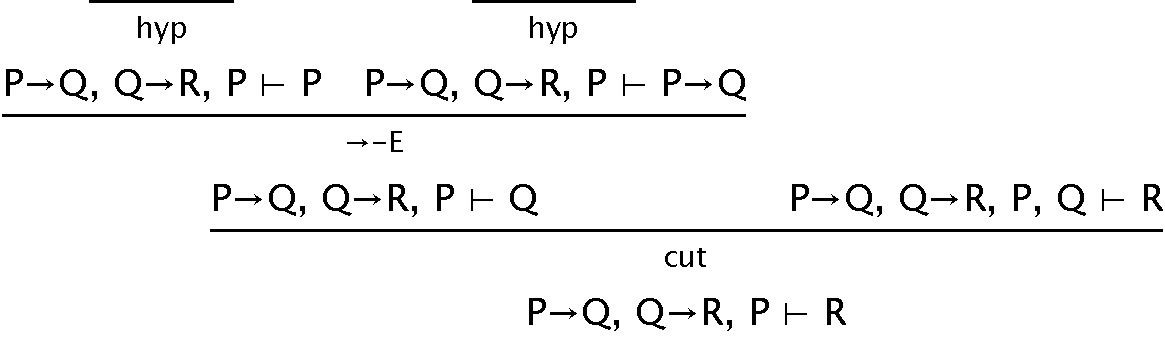
\includegraphics[scale=0.5]{pics/treeforwardstepwithcutC} \label{fig:treeforwardstepwithcutC}} 
%\quad
%\subfigure[after second →-E]{\centering
%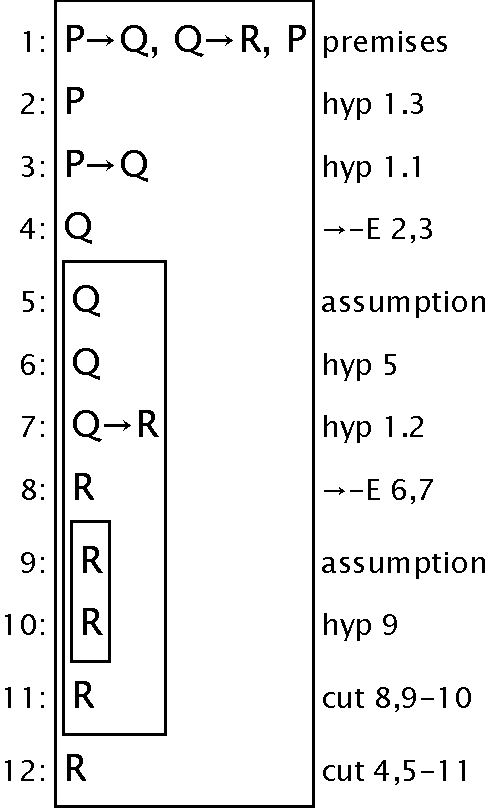
\includegraphics[scale=0.5]{pics/forwardstepwithcutE} \label{fig:forwardstepwithcutE}} 
%\quad
%\subfigure[tree after second →-E]{\centering
%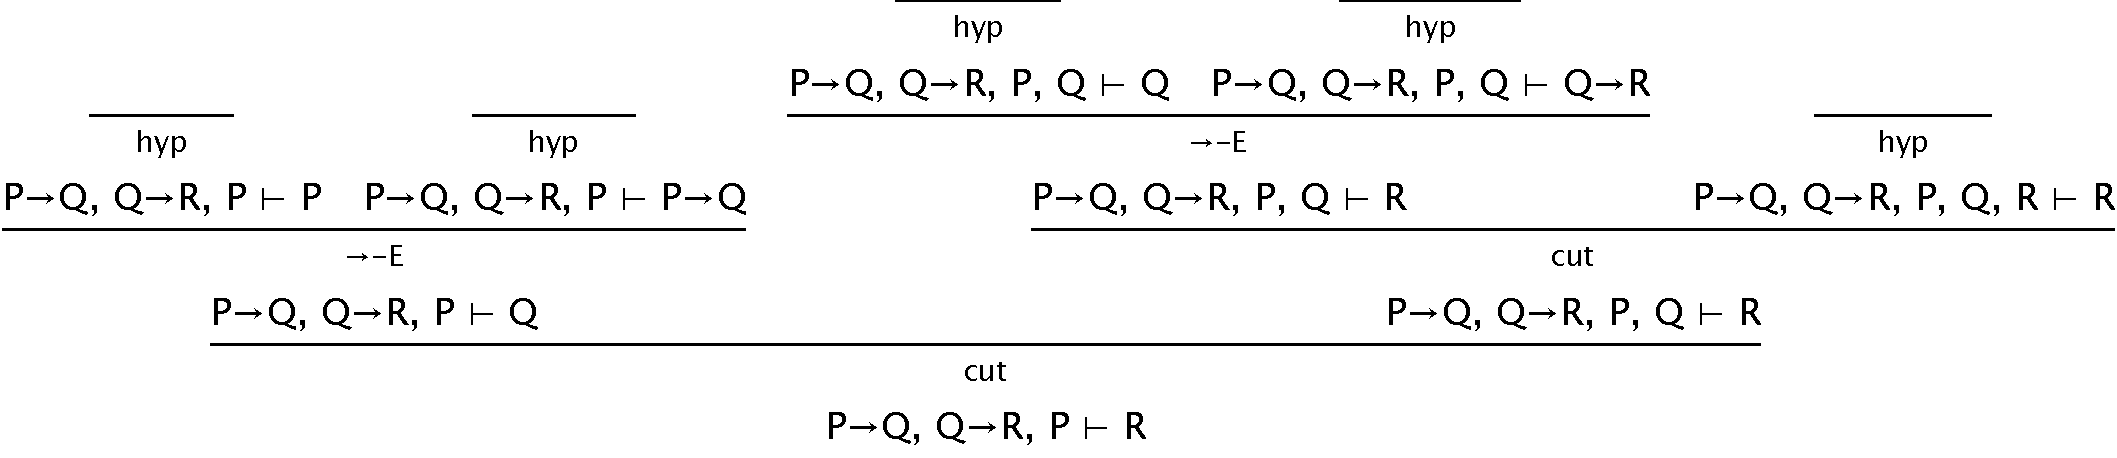
\includegraphics[scale=0.5]{pics/treeforwardstepwithcutE} \label{fig:treeforwardstepwithcutE}} 
\caption{A proof using forward steps, showing \texttt{cut} and \texttt{hyp}}
\label{fig:forwardstepwithcut}
\end{figure}

\begin{figure} 
\centering 
\subfigure[the problem]{\centering
\fbox{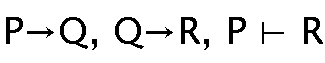
\includegraphics[scale=0.5]{pics/forwardstepslowlyA}} \label{fig:forwardstepslowlyA}} 
\quad
\subfigure[after \texttt{cut}, with unknown $\_B$]{\centering
\fbox{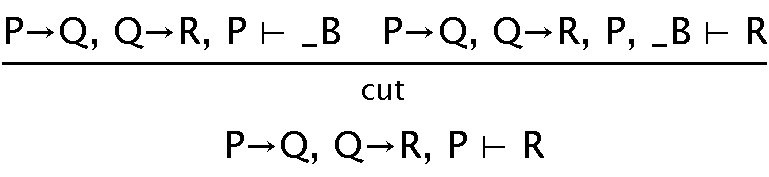
\includegraphics[scale=0.5]{pics/forwardstepslowlyB}} \label{fig:forwardstepslowlyB}} 
\quad
\subfigure[after →-E, with unknowns $\_A$ and $\_B$]{\centering
\fbox{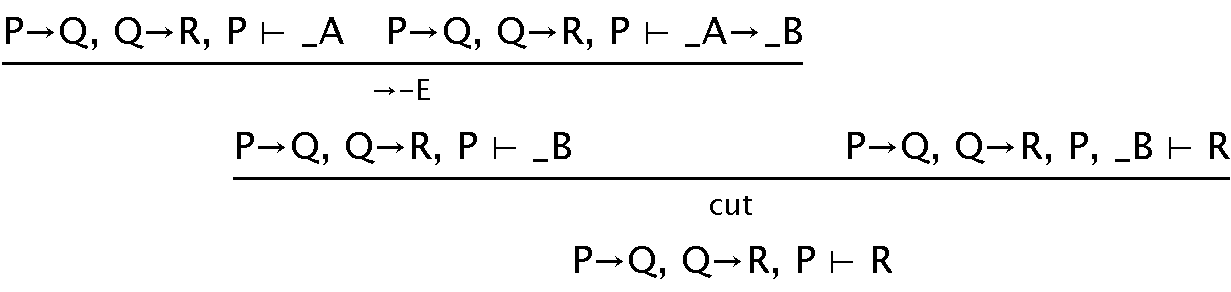
\includegraphics[scale=0.5]{pics/forwardstepslowlyC}} \label{fig:forwardstepslowlyC}} 
\quad
\subfigure[after first \texttt{hyp} (from user selection)]{\centering
\fbox{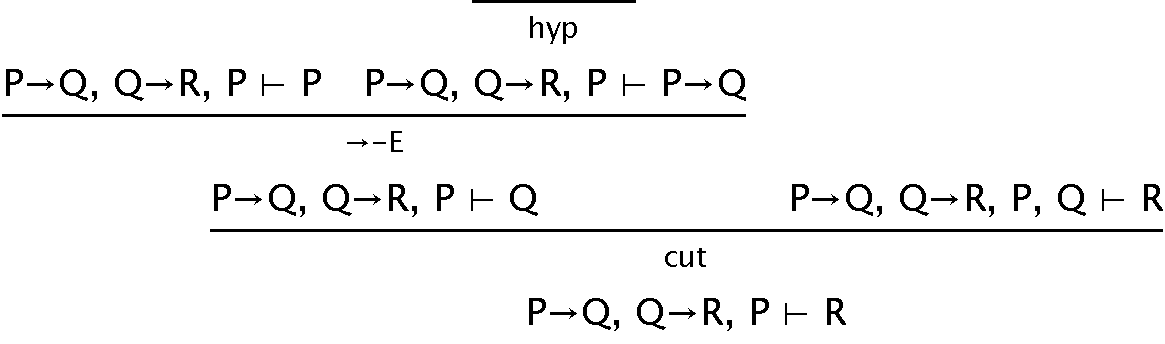
\includegraphics[scale=0.5]{pics/forwardstepslowlyD}} \label{fig:forwardstepslowlyD}} 
\quad
\subfigure[after second \texttt{hyp} (by \textsc{automatch})]{\centering
\fbox{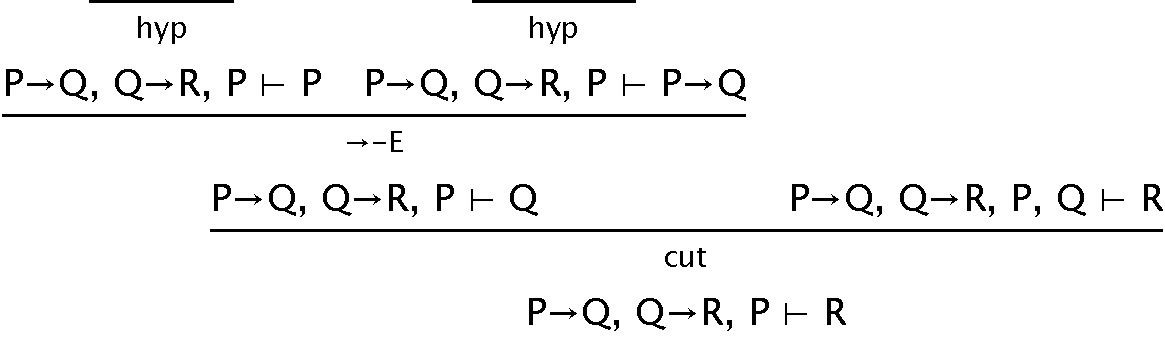
\includegraphics[scale=0.5]{pics/forwardstepslowlyE}} \label{fig:forwardstepslowlyE}} 
\caption{Stages of a sample `forward step'}
\label{fig:forwardstepslowly}
\end{figure}

\section{Forward reasoning with \texttt{cut}}

The sort of steps that a natural-deduction reasoner might want to make is best illustrated by example. Consider the problem of proving $P->Q, Q->R, P |- R$, the second problem in the Conjectures panel defined in \texttt{ItL\_problems.j}. \Figref{forwardstepA} shows the initial display; \ref{fig:forwardstepB} the first selection; \ref{fig:forwardstepC} the effect of →-E; \ref{fig:forwardstepD} the second selection; \ref{fig:forwardstepE} the effect of a second application of →-E. 

The proof is complete, and has apparently used forward reasoning. Yet in fact it was all done with backward reasoning, and the logic has only right-hand rules --- nothing that can work on hypotheses.

The magic is all done with the \texttt{hyp} and \texttt{cut} rules. If you set the \texttt{hidehyp} and \texttt{hidecut} variables to \texttt{false}, the first step goes as in \figref{forwardstepwithcutC}: a couple of \texttt{hyp} steps move $P$ and $P->Q$ from left to right, making them available for the →-E step; then →-E extracts $Q$; then a \texttt{cut} step moves $Q$ from right to left, making it available as a hypothesis to prove $R$. With \texttt{hyp} steps hidden lines 1 and 2 disappear. We are left with the pattern on lines 4, 5, 6 and 7: a \texttt{cut} whose left arm is proved by a rule step, and whose conclusion is the same as the right arm of the cut. Such a pattern can be expressed as a single line: add a hypothesis labelled for the rule step, as in \figref{forwardstepC}.

In fact the proof has to be built backwards, as you can see from the tree in \figref{treeforwardstepwithcutC}: \texttt{cut}, →-E, \texttt{hyp}, \texttt{hyp} . Jape uses unknowns in every step until the \texttt{hyp}s make it all concrete. The steps are shown in \figref{forwardstepslowly}: note that the first \texttt{hyp} in \figref{forwardstepslowlyD} eliminates both the unknowns, so that the second \texttt{hyp} can proceed unprompted, by matching rather than unification.

The mechanism is invoked by the →-E entry in the Rules menu:
\begin{quote}\tt\small
MENU Rules IS
    ENTRY "→-I" \\
    ENTRY "∧-I"    \\
    ENTRY "∨-I(L)"  IS ForwardOrBackward ForwardCut 0 "∨-I(L)"\\
    ENTRY "∨-I(R)"  IS ForwardOrBackward ForwardCut 0 "∨-I(R)"\\
    ENTRY "¬-I"\\
    ENTRY "∀-I"\\
    ENTRY "∃-I"     IS "∃-I with side condition hidden"\\
    SEPARATOR\\
    ENTRY "→-E"     IS ForwardOrBackward ForwardCut 1 "→-E" \\
    ENTRY "∧-E(L)"  IS ForwardOrBackward ForwardCut 0 "∧-E(L)"\\
    ENTRY "∧-E(R)"  IS ForwardOrBackward ForwardCut 0 "∧-E(R)"\\
    ENTRY "∨-E"     IS ForwardOrBackward ForwardUncut 0 "∨-E"  \\ 
    ENTRY "¬-E"     IS ForwardOrBackward ForwardCut 0 "¬-E" \\
    ENTRY "∀-E"     IS ForwardOrBackward ForwardCut 0 "∀-E with side condition hidden"\\  
    ENTRY "∃-E"     IS ForwardOrBackward ForwardUncut 0 "∃-E"\\
    SEPARATOR\\
    ENTRY hyp
END
\end{quote}

\var{rule}
\texttt{ForwardOrBackward} detects whether to use a forward or a backward step:\footnote{For no good reason that I can recall, tactics and rules are applied ``Curried'' style as $t\; a_{1}\;a_{2}\;...$ but defined with tuple arguments as $t\; (a_{1},\;a_{2},\;...)$.}
\begin{quote}\tt\small
TACTIC ForwardOrBackward (Forward, n, rule) IS \\
\tab WHEN    \\
\tab \tab (LETHYP \_P \\
\tab \tab \tab (ALT    \\
\tab \tab \tab \tab (Forward n rule)\\
\tab \tab \tab \tab (WHEN   \\
\tab \tab \tab \tab \tab (LETARGSEL \_Q \\
\tab \tab \tab \tab \tab \tab (Fail (rule is not applicable to assumption ' \_P ' with argument ' \_Q ')))\\
\tab \tab \tab \tab \tab (Fail (rule is not applicable to assumption ' \_P ')))))\\
\tab \tab (ALT    \\
\tab \tab \tab (WITHSELECTIONS rule)\\
\tab \tab \tab (WHEN   \\
\tab \tab \tab \tab (LETARGSEL \_P\\
\tab \tab \tab \tab \tab (Fail (rule is not applicable with argument ' \_P ')))\\
\tab \tab \tab \tab (Fail (rule is not applicable))))
\end{quote}
Stripped to its bones, without the error-handling code, this tactic is
\begin{quote}\tt\small
TACTIC ForwardOrBackward (Forward, n, rule) IS \\
\tab WHEN  \\
\tab \tab (LETHYP \_P (Forward n rule))\\
\tab \tab (WITHSELECTIONS rule)
\end{quote}
\textsc{when} takes the first of its arguments whose guard succeeds. \textsc{lethyp} $\_P$ succeeds if the user has selected a hypothesis which matches $\_P$ --- i.e. any hypothesis at all. \texttt{Forward} $n$ $\<rule>$ does the work in that case. If \textsc{lethyp} doesn't match, it's a backward step and \textsc{withselections} $\<rule>$ does the work instead.

In the full tactic, \textsc{alt} applies its arguments in turn until one succeeds, and fails if none succeed. If \texttt{Forward} fails in the forward-step arm, you get a message generated by \texttt{Fail} which varies according to whether or not you have subformula-selected $\_Q$ (the messages are somewhat archaicly constructed: later chapters will show how to make them more nicely), and similarly in the backward-step arm (with slightly different messages).

The \texttt{Forward} argument is in fact \texttt{ForwardCut}, $n$ is 1 and $\<rule>$ is \texttt{"→-E"}. \texttt{ForwardCut} applies \texttt{cut} and then \texttt{ForwardUncut}:
\begin{quote}\tt\small
TACTIC ForwardCut (n,rule) \\
\tab SEQ cut (ForwardUncut n rule)
\end{quote}

\texttt{ForwardUncut} applies the rule and then applies \texttt{hyp} to the $n$th antecedent:
\begin{quote}\tt\small
TACTIC ForwardUncut (n,rule) \\
\tab (LETGOALPATH G \\
\tab \tab (WITHARGSEL rule) \\
\tab \tab (GOALPATH (SUBGOAL G n)) \\
\tab \tab (WITHHYPSEL hyp) \\
\tab \tab (GOALPATH G) \\
\tab \tab NEXTGOAL)
\end{quote}
\textsc{letgoalpath} binds $G$ to the current position in the tree and then applies its arguments as a \textsc{seq} tactic. \textsc{withargsel} $\<rule>$ applies $\<rule>$ (\texttt{"→-E"} in our case), with the user's subformula selections, if any, as the first argument (see sections \ref{sec:basics:gestures} and \ref{sec:basics:parameters}). Then it goes to the $n$th antecedent of the tree that $\<rule>$ generates and applies \texttt{hyp}, using the user's selected hypothesis. A rule uses the user's selections to disambiguate alternative rule matches: in this case the hypothesis selection picks out one left-hand formula for \texttt{hyp} to work on. Finally the tactic goes back to the base of the subtree it's built and moves (\textsc{nextgoal}) to its leftmost tip, or if the tree is closed to the next available tip in the tree.

If the user doesn't select a hypothesis, \textsc{withselections} in \texttt{ForwardOrBackward} applies $\<rule>$, taking account of the user's conclusion and subformula-selections (if any).

Finally, as we've seen, \textsc{automatch} tidies up.

\section{Other menu entries}

Two of the entries in the Rules menu give a tactic as argument to \texttt{ForwardorBackward}, not a rule. The tactics in question are:
\begin{quote}\tt\small
TACTIC "∀-E with side condition hidden" IS \\
\tab LAYOUT "∀-E" (0) (WITHARGSEL "∀-E")\\
TACTIC "∃-I with side condition hidden" IS \\
\tab LAYOUT "∃-I" (0) (WITHARGSEL "∃-I")
\end{quote}
The \textsc{layout} tactical takes a tuple describing the arguments which ought to be visible: here it's (0), which means that antecedent 1, the $c\;\<inscope>$ antecedent, is hidden. The rest of its arguments are a sequence of tactics: I have to reapply \textsc{withargsel} to make the rule sensitive to the user's argument selection.

As in chapter 3, there is a rule for the $\<inscope>$ judgement, which is tried at the end of every proof step:
\begin{quote}\tt\small
RULE "inscope" IS INFER var x ⊦ x inscope \\
AUTOMATCH "inscope"
\end{quote}

\section{Automatic rule selection (\texttt{ItL\_hits.j})}

There is a file ItL\_hits.j, which implements double-clicking in this encoding: I didn't reference this in ItL.jt, because I  didn't want to provide it by default to novices.

\section{The Conjectures panel (\texttt{ItL\_problems.j})}

Since we can apply rules either forward or backward, it would be irksome if we could only apply theorems backward. I define a tactic which can do the job. If a hypothesis has been selected it cuts and applies the theorem, requiring that the selected hypothesis be one of the principal formulae which match the theorem sequent. If no hypothesis is selected it tries in order to apply the theorem to the present problem sequent, to apply it `by resolution' (matching only the right-hand side of the theorem sequent and the problem sequent and generating antecedents for each left-hand side theorem formula: see \secref{basics:application}), and finally tries to apply it forwards, one way or the other. All of the steps are made `\textsc{withselections}' --- that is, using any hypothesis, conclusion or subformula-selection which the user may have made:
\begin{quote}\tt\small
TACTIC TheoremForwardOrBackward(thm) IS\\
\tab WHEN \\
\tab \tab (LETHYP \_P cut (WITHSELECTIONS thm))\\
\tab \tab (ALT \\
\tab \tab \tab (WITHSELECTIONS thm) \\
\tab \tab \tab (RESOLVE (WITHSELECTIONS thm)) \\
\tab \tab \tab (SEQ cut (ALT (WITHSELECTIONS thm) (RESOLVE (WITHSELECTIONS thm)))) \\
\tab \tab )
\end{quote}

The overall effect is to allow a prover to introduce a theorem into the proof whenever it is helpful to do so.\\
The Conjectures panel activates this tactic from its Apply button:
\begin{quote}\tt\small
CONJECTUREPANEL Conjectures\\
\tab THEOREM INFER P, P → Q ⊦ Q\\
\tab THEOREM INFER P → Q, Q → R, P ⊦ R\\
\tab THEOREM INFER P → (Q → R), P → Q, P ⊦ R

\tab ...

\tab THEOREM "(∀x.P(x)) → (∀x.Q(x)) ⊦ ∀x.(P(x) → Q(x)) NOT" IS ∀x.P(x) → ∀x.Q(x) ⊦ ∀x.(P(x) → Q(x))\\
\tab THEOREM "(∃x.P(x)) ∧ (∃x.Q(x)) ⊦ ∃x.(P(x) ∧ Q(x)) NOT" IS ∃x.P(x) ∧ ∃x.Q(x) ⊦ ∃x.(P(x) ∧ Q(x))

\tab BUTTON Apply IS apply TheoremForwardOrBackward COMMAND \\
END
\end{quote}
(Most conjectures are named by their sequent, but the last few are specially named because a proof attempt is certain to fail.)

When the Apply button is pressed with a conjecture $C$ selected, the effect is to send the command ``apply TheoremForwardOrBackward $C$ '' to theproof engine.

\section{Other natural deduction encodings}

Bernard's J'n'J encoding is in \texttt{examples/jnj}, and described in ``Using J'n'J in Jape'', distributed with Jape. My own encoding is in \texttt{examples/natural\_deduction}, is described in my book (\textit{An Introduction to Proof and Disproof in Formal Logic}, OUP 2005) and dissected in \chapref{I2L} below.
 